\documentclass[10pt,a4paper]{article}
\usepackage{hyperref}
\usepackage[a4paper, total={6in, 10in}]{geometry}
\usepackage[LGR]{fontenc}
\usepackage[utf8]{inputenc}
\usepackage[greek]{babel}
\usepackage{graphicx}
\graphicspath{ {./images/} }

\title{ Γραφική με Υπολογιστές \\ -Εργασία \textlatin{\#}2-}
\author{Θωμάς Πλιάκης \\ \textlatin{tpliakis@ece.auth.gr} \\ AEM: 9018}
\date{\today}

\begin{document}
\maketitle

\section*{\textlatin{interpolate\_color}}
Η συνάρτηση \textbf{\textlatin{vector\_interp}} υλοποιεί πολύ απλά μια γραμμική παρεμβολή μεταξύ των σημείων που δίνονται ως ορίσματα με τον παρακάτω τρόπο:

\[r1 = ||x2-x||\]   
\[r2 = ||x-x1||\]
\[percent = \frac{r1}{r1 +r2}\]
\[value = percent*C1+(1-percent)*C2\]

Όπου \textlatin{r1} και \textlatin{r2} είναι οι απόστασεις των ενεργών σημείων από το σημείο της παρεμβολής, \textlatin{r1 + r2} είναι η απόσταση των σημείων \textlatin{x1}, \textlatin{x2}. Με την διαίρεση γίνεται μια κανονικοποίηση για να έχουμε το ποσοστό μεταξύ 0 και 1 που πρέπει να συμμετέχει κάθε σημείο στον χρωματισμό. 

Ο κώδικας, λόγω της βιβλιοθήκης \textbf{\textlatin{numpy}} μπορεί να υλοποιεί την γραμμική παρεμβολή με μεταβλητές οποιονδήποτε διαστάσεων.


\section*{\textlatin{shade\_triangle}}
Επειδή η υλοποίηση των δύο \textbf{\textlatin{mode ,["flat" , "gouraud"]}}, ξεκίνησε διαφορετκά, η ενοποιήση των 2 διαδικασιών έγινε με ένα \textbf{\textlatin{if ... else}} ανάλογα το όρισμα \textbf{\textlatin{shade\_t}}.

Η συνάρτηση \textbf{\textlatin{shade\_triangle}} με όρισμα \textbf{\textlatin{shade\_t = "flat"}} αποδίδει ένα χρώμα σε κάθε τρίγωνο, τον μέσο όρο των χρωμάτων των κορυφών του. Τα βήματα του αλγορίθμου περιγράφονται παρακάτω: 
\begin{enumerate}
    \item Υπολογισμός και αποθήκευσή του μέσου όρου των χρωμάτων στον 1\textlatin{x}3 πίνακα \textbf{\textlatin{c}}.
    \item Υπολογισμός των ελάχίστων και μεγίστων συντεταγμένων της κάθε πλευράς,  καθώς και της κλίσης τους, \textbf{\textlatin{Ykmin,Xkmin,Ykmax,Xkmax}}.
    \item Εύρεση των ολικών μεγίστων και ελαχίστων συντεταγμένων του τριγώνου, \textbf{\textlatin{Ymin,Xmin,Ymax,Ymin}}.
    \item Βρίσκουμε ποιες είναι οι αρχικές ενεργές πλευρές(παίρνουν το λογικό 1) και αποθηκεύουμε σε πίκανκα τις συντεταγμένες τους, που αποτελούν και τα ενεργά οριακά τους σημεία \textbf{\textlatin{ActiveSides,Xk}}. Στον πίνακα \textbf{\textlatin{Xact}} αποθηκεύονται οι τετμημένες των 2 ενεργών σημείων μόνο.
    \item Μπαίνουμε στην κυρίως επανάληψη στην οποία:
    \begin{itemize}
        \item Ελέγχουμε αν βρισκόμαστε σε κορυφή του τριγώνου.
        \item Υλοποιείται το σκανάρισμα σε όλες τις τετμημένες για συγκεκριμένη τεταγμένη κατά την οποία αν κάποιο \textbf{\textlatin{pixel}} βρίσκεται μέσα ή πάνω στο τρίγωνο χρωματίζεται.
        \item Ενημερώνεται η λίστα των ενεργών πλεύρων.
        \item Τέλος ενημερώνεται η λίστα με τα νέα ενεργά σημεία ανάλογα με την κλίση της κάθε πλευράς του τριγώνου.
      \end{itemize}
  \end{enumerate}


H συνάρτηση \textbf{\textlatin{shade\_triangle}} με όρισμα \textbf{\textlatin{shade\_t = "gouraud"}} έκτελεί τις ίδιες αρχικοποιήσεις με προηγουμένως αλλά και κάποιες ακόμα. Τα επιπλέον βήματα του αλγορίθμου που γίνονται είναι:
\begin{enumerate}
    \item Αποθηκεύση των δεικτών των κορυφών κάθε ακμής στις λίστες \textbf{\textlatin{minindex, maxindex}}.
    \item Αποθηκεύση των δεικτών των 2 ενεργών σημείων κάθε ακμής στις λίστα \textbf{\textlatin{index}} για προσέλαση των \textbf{\textlatin{colorsAct}}, \textbf{\textlatin{Xact}} πινάκων.
    \item Αποθηκεύση του χρώματος των ενεργών οριακών σημείων στην λίστα  \textbf{\textlatin{colorsAct}}.
    \item Όταν γίνεται ο χρωματσμός κάποιου σημείου εσωτερικά του τριγώνου, υπολογίζεται το χρώμα του από την \textbf{\textlatin{interpolate\_color}} και τα 2 ενεργά σημεία. 
    \item Ο υπολογισμός του χρώματος για τα ενεργά οριακά σημεία γίνεται με χρήση της \textbf{\textlatin{interpolate\_color}} από τις αντίστοιχες κορυφές κατά την ενημέρωση της λίστας με τα ενεργά σημεία.
\end{enumerate}

Όλα τα παραπάνω γίνονται για τον χρωματισμό ενός αντικειμένου
ολόκληρου που αποτελείται από πολλά τρίγωνα. Αυτό γίνεται στην συνάρτηση:

\section*{\textlatin{render}}
Ο κώδικας στην συνάρτηση \textbf{\textlatin{render}} περιγράφεται στα παρακάτω βήματα:

\begin{enumerate}
    \item Γίνεται υπολογισμός του βάθους του κάθε τριγώνου, \textbf{\textlatin{Dm}}.
    \item Ταξινομώ τον πίνακα αυτό κατά φθίνουσα σειρά. Με την ίδια σειρά ταξινομείται και ο πίνακας \textbf{\textlatin{faces}}, με την βοήθεια του \textbf{\textlatin{D\_order}} που περίεχει την σειρά που ταξινομήθηκε ο \textbf{\textlatin{Dm}}.
    \item Ανάλογα με ποιο από τα 2 \textbf{\textlatin{mode}} θέλουμε να χρησιμοποιήσουμε, επιλέγουμε την κατάλληλη τιμή για την μεταβλητή  \textbf{\textlatin{shade\_t ,["flat" , "gouraud"]}}.
 \end{enumerate}

\section*{Σχόλια}
\begin{itemize}
  \item Τέλος δεν έγινε καμία άλλη παραδοχή πέρα από αυτές της εκφώνησης και των σημειώσεων που περιγράφουν των αλγόριθμο που κληθήκαμε να υλοποιήσουμε.
  χρόνος αφού ο κώδικάς δεν παράγει ακριβώς τον σωστό αποτέλεσμα.
\end{itemize}


\section*{Αποτελέσματα της \textlatin{shade\_t = "flat"}:} 

\includegraphics[scale=0.8]{flat.png}

\section*{Αποτέλεσμα της \textlatin{shade\_t = "gouraud"}:}
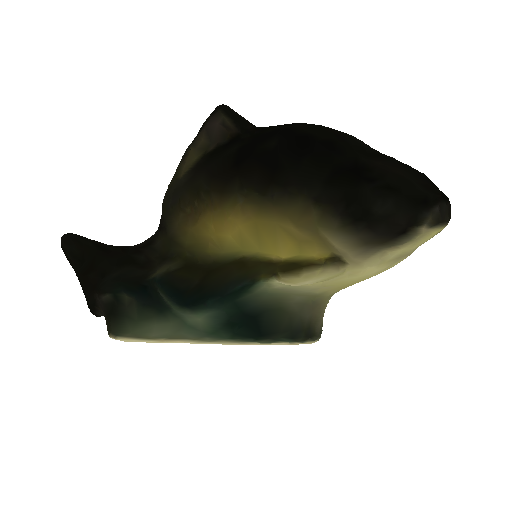
\includegraphics[scale=0.8]{gouraud.png}
\end{document}